\documentclass{article}
\usepackage[utf8]{inputenc}
\usepackage{amsmath}
\usepackage{amsfonts}
\usepackage{graphicx}
% \usepackage{gensymb}
\title{Discussion Assignment Unit 7\\
Math 1201 - College Algebra.
}
\author{Jasper Albert Nri}
\date{October 2021}


\begin{document}

\maketitle

\section*{PART 1}
\title\textbf{QUESTION}\\
Given two similar triangles, one with small measurements that can be accurately determined, and the other with large measurements, but at least one is known with accuracy, can the other two measurements be deduced? Explain and give an example.\\
\\\title\textbf{Solution}\\
Given two triangles a small one and a large one the way to find out if both triangles are similar to each other is by using pythagoras theorem.\\
\\\title\textbf{Small triangle}
\\Given a triangle with three sides a, b, and c.
\\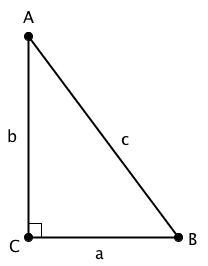
\includegraphics[scale = 0.35]{abc}\\
where,\\
a = 3,\\
b = 4,\\
c = 5.\\
The angles within the triangle can be determined using SOH CAH TOA.
So for the triangle given above the angle B can be determined with this method.
$${\sin B = \frac{opp}{hyp}}$$
$${\sin B = \frac{4}{5}}$$
$${B =\sin^{-1}{{\frac{4}{5}}}}$$
$${B = 53.13^{\circ}}$$
Now the sum of angles within a triangle is ${180^{\circ}}$ and since this is a right-angled triangle,
${C = 90^{\circ}}$, then  
$${180 = A+B+C}$$
$${A = 180-B-C}$$
$${A = 180-53.13-90}$$
$${A = 180-143.13}$$
$${A = 36.87^{\circ}}$$

So for a small right-angled triangle whose sides have been accurately determined, the angles of the other sides can be determined using SOH CAH TOA technique.\\
\\\title\textbf{Large triangle}
\\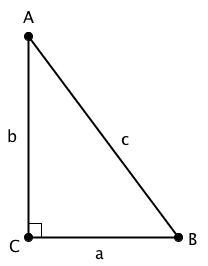
\includegraphics[scale = 0.65]{abc}\\
Given a single side of a large right angled triangle and it's correponding opposite angle the other two sides of the triangle can be found, using SOH CAH TOA and pythagoras theorem.
if c = ?, a = ?, b = 12 and ${B = 67.38^{\circ}}$.
\\recall pythagoras theorem for this triangle is 
$${c = \sqrt{a^2 + b^2}}$$
But also Using SOH, 
$${\sin B  = \frac{b}{c}}$$
but ${c = \sqrt{a^2 + b^2}}$,  B = 67.38, and b = 12, substituting
$${\sin (67.38)  = \frac{12}{\sqrt{a^2 + 12^2}}}$$
cross Multiply to make a subject
$${  \sqrt{a^2 + 144}= \frac{12}{\sin (67.38)}}$$
Take the square of both sides 
$${\left(\sqrt{a^2 + 144}\right)^2= \left(\frac{12}{0.9231}\right)^2}$$
$${a^2 + 144 = \frac{144}{0.8521}}$$
$${a^2 + 144 = 169}$$
$${a^2 = 169 - 144}$$
$${a^2 = 25}$$
$${a = \sqrt{25}}$$
$${a = 5}$$

If you can recall ${c = \sqrt{a^2 + b^2}}$, since a = 5, and b = 12, 
$${c = \sqrt{a^2 + b^2}}$$
$${c = \sqrt{5^2 + 12^2}}$$
$${c = \sqrt{25 + 144}}$$
$${c = \sqrt{169}}$$
$${c = 13}$$

So therefore using pythagoras theorem and SOH CAH TOA, we have been able to determine the other two sides of a right angled triangle.\\
\\\title\textbf{Determine Similarity}
Let's use the small triangle as an example,\\
The small triangle has sides of length 3, 4, and 5 units, if this was to be scaled by a factor of 100 to give a new large triangle, we can determine if the small triangle is similar to the newly scaled triangle by taking the ratio of the sides in each traingle and comparing it.\\
Example:
For small triangle, a = 3, b = 4, c = 5, and for new large triangle a = 300, b = 400, c = 500
\\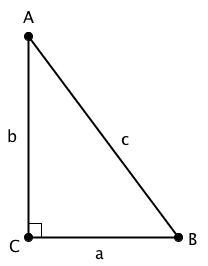
\includegraphics[scale = 0.55]{abc}\\
if the ratio of ${\frac{a}{b}}$ for small triangle is equal to the ratio of ${\frac{a}{b}}$ for the newly created large triangle then we can say that the two triangles are similar.
To check, ratio for ST,
$${ratio = \frac{a}{b}}$$  
$${ratio = \frac{3}{4}}$$  
$${ratio = 0.75}$$
To check for LT,  
$${ratio = \frac{a}{b}}$$  
$${ratio = \frac{300}{400}}$$  
$${ratio = 0.75}$$  
ratio of ST = ratio of LT.\\
Therefore the two triangles are similar.\\
\\\title\textbf{SUMMARY}\\
From the examples given and illustrated above, i have demonstrated how the angles of a right triangle can be derived when given all the sides using the SOH CAH TOA method and trigonometric inverses(Abramson,2017)..\\
I also demonstrated how the other two sides of a right triangle can be gotten when given one side and an angle, using SOH CAH TOA and the pythagoras theorem(Abramson,2017)..\\
Lastly I also showed that one of the best ways to check for similarities between two right-angled triangle is by taking the ratios of the sides of each triangle and comparing them with their respective counterpart(Abramson,2017).



\section*{PART 2}
\title\textbf{QUESTION}\\
How could we understand that the right triangles of trigonometry with a hypotenuse of measure 1, represent all possible right triangles?\\
\\\title\textbf{Solution}\\
There are two distinct configurations of all possible right triangle and they can be modelled with a hypotenuse of measure 1.\\
Below i will illustrate each configurations with Using a hypotenuse of measure 1.
\\\title\textbf{Configuration 1}\\
In this case, the other sides of the right triangle are equal.
\\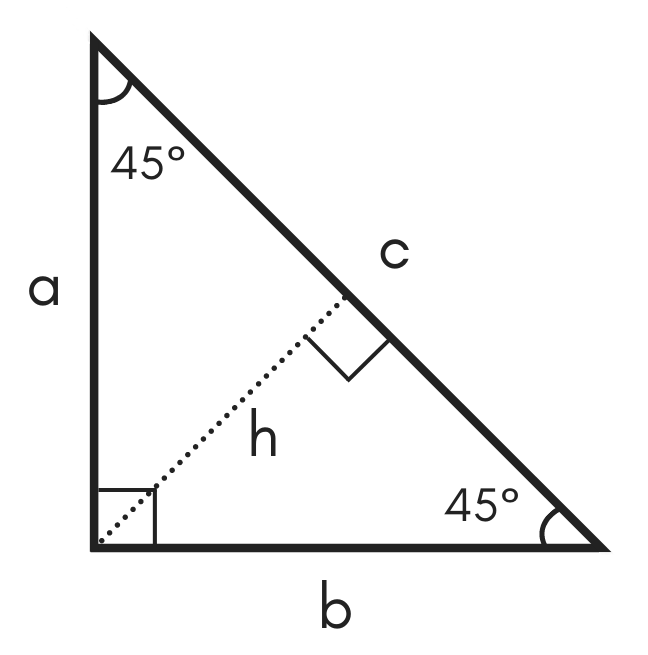
\includegraphics[scale = 0.25]{45}\\
By pythagoras theorem ${c^2=a^2+b^2}$ 
Where c is the hypotenuse and a and b are the two other sides. These two sides are equal, so therefore, ${a^2 = b^2}$.
Rewriting the pythagoras theorem.
$${c^2 = a^2+b^2}$$
$${c^2 = a^2+a^2}$$
$${c^2 = 2a^2}$$ 
divide both sides by 2
$${a^2 = \frac{c^2}{2}}$$ 
Take the square root of both sides 
$${\sqrt{a^2} = \sqrt{\left(\frac{c^2}{2}\right)}}$$ 
$${a = \frac{c}{\sqrt{2}}}$$ 
Recall c = 1\\
Rationalizing, 
$${a = \frac{1}{\sqrt{2}} \times \frac{\sqrt{2}}{\sqrt{2}}}$$ 

$${a = \frac{\sqrt{2}}{2}}$$ 

For a right angled-triangle with a hypotenuse of 1, if the two sides are the same then the sides are given as ${\frac{\sqrt{2}}{2}}$ and the general format or model that can be used to get these sides using the pythagoras theorem is $${c^2 = 2a^2}$$ 
Where c is the hypotenuse and a is one of the other side.\\
\\\title\textbf{Configuration 2}\\
In this case, none of the sides of the right triangle are equal.
\\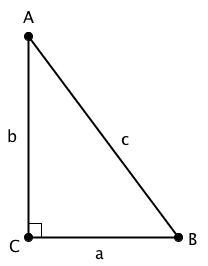
\includegraphics[scale = 0.55]{abc}\\
By pythagoras theorem ${c^2=a^2+b^2}$ 
if ${a = \frac{1}{2}}$, then b can be gotten using pythagoras theorem.
$${c^2=a^2+b^2}$$
$${1^2 = \left(\frac{1}{2}\right)^2 + b^2}$$
$${b^2 = 1^2 - \left(\frac{1}{2}\right)^2}$$
$${b^2 = 1 - \frac{1}{4}}$$
$${b^2 = \frac{3}{4}}$$
Taking the square root of both sides
$${b = \sqrt{\frac{3}{4}}}$$
$${b = \frac{\sqrt{3}}{2}}$$

So for a right angled triangle with hypotenuse 1 and one of the sides is ${\frac{1}{2}}$, the third side is given as  ${\frac{\sqrt{3}}{2}}$ as determined by the pythagorean theorem.\\
\\\title\textbf{Summary}\\
For a right angled triangle with a hypotenuse of 1 unit there are two possible configurations in which it can be represented,\\
The first is when the other two sides are equal, this usually translates to a angle of ${45^{\circ}}$ between the other two sides and the hypotenuse. The value of the two sides can be determined using pythagoras theorem or the SOH CAH TOA method(Abramson,2017)..\\
The second is when all three sides are not equal, here the sides can be determined using the combination of pythagoras theorem and the SOH CAH TOA (Abramson,2017).\\




\section*{References}
Abramson, J. (2017). \textit{Algebra and trigonometry}. OpenStax, TX: Rice University. Retrieved
from https://openstax.org/details/books/algebra-and-trigonometry
\end{document}